\begin{figure}[H]
    \centering
    
    \tikzset{
    state/.style={circle,draw,inner sep=5},
    win/.style={circle,draw,inner sep=2},
    loss/.style={circle,draw,inner sep=2, fill=black}
    }
    
    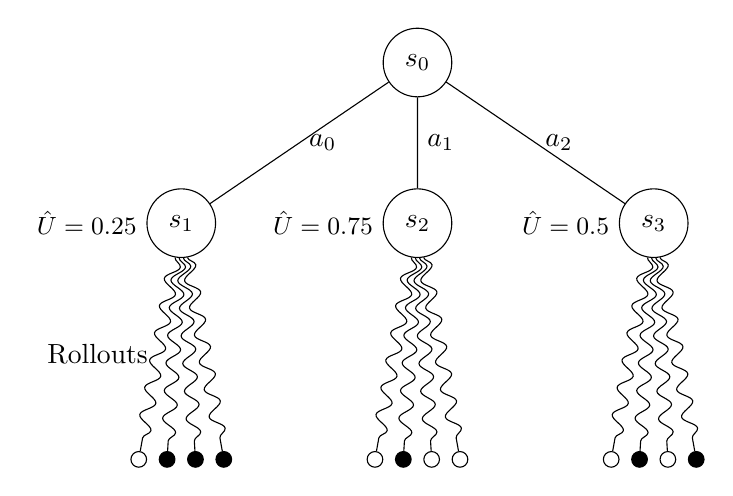
\begin{tikzpicture}[scale=12]
    % Specify spacing for each level of the tree
    \tikzstyle{level 1}=[level distance=1.7mm,sibling distance=2.5mm]
    \tikzstyle{level 2}=[level distance=2.5mm,sibling distance=.3mm]
    % The Tree
    \node(0)[state]{$s_0$}
    child{node[state, label=left:{\small $\hat{U}=0.25$}]{$s_1$}
    child{node[win]{}
        edge from parent[decorate, decoration=snake] node[left]{Rollouts}
        }
        child{node[loss]{}
        edge from parent[decorate, decoration=snake]
        }
        child{node[loss]{}
        edge from parent[decorate, decoration=snake]
        }
        child{node[loss]{}
        edge from parent[decorate, decoration=snake]
        }
        edge from parent node[right]{$a_0$}
    }
    child{node[state, label=left:{\small $\hat{U}=0.75$}]{$s_2$}
        child{node[win]{}
        edge from parent[decorate, decoration=snake]
        }
        child{node[loss]{}
        edge from parent[decorate, decoration=snake]
        }
        child{node[win]{}
        edge from parent[decorate, decoration=snake]
        }
        child{node[win]{}
        edge from parent[decorate, decoration=snake]
        }
        edge from parent node[right]{$a_1$}
    }
    child{node[state, label=left:{\small $\hat{U}=0.5$}]{$s_3$}
        child{node[win]{}
        edge from parent[decorate, decoration=snake]
        }
        child{node[loss]{}
        edge from parent[decorate, decoration=snake]
        }
        child{node[win]{}
        edge from parent[decorate, decoration=snake]
        }
        child{node[loss]{}
        edge from parent[decorate, decoration=snake]
        }
        edge from parent node[right]{$a_2$}
    };

    \end{tikzpicture}

    \caption{The simplest Monte Carlo method, with a budget of 12 total
    rollouts. White leaf nodes
    corresponds to wins, and black to losses. Action $a_1$ maximizes
    the average utility $\hat{U}$ at 0.75, and is therefore the move chosen.}
    \label{fig:simple_monte_carlo}

\end{figure}